%!TEX root = ../thesis.tex

\section{Appendix: Unused theorems}


\begin{thrm}
\label{th:irreducible and chordfree triangulation of the kgon is 3connected}
A irreducible triangulation $G$ of the $k$-gon with a chordfree outer cycle is $3$-connected.
\end{thrm}
\begin{proof}
  This proof has to be expanded.

  The completion $G'$ is a irreducible triangulation. Chordfree outer cycle is important, because a chord will form a separating triangle in $G'$.
\end{proof}

\begin{thrm}
  Any irreducible triangulation $T$ of the $4$-gon with $n \geq 5$ is $3$-connected.
\end{thrm}
\begin{proof}
  Let us name the four vertices of the outer cycle $a,b,c,d$, this cycle has at least one interior vertex $v$ since $n\geq 5$. The edges $ac$ and $bd$ can't exist since they would create a separating triangle containing $v$. hence the outer cycle is chordfree.
  Theorem \ref{th:irreducible and chordfree triangulation of the kgon is 3connected} then concludes the proof
\end{proof}


\begin{thrm}
  Every interior vertex of a triangulation of the $n$-gon has degree at least $3$.
\end{thrm}

\begin{proof}
  This follows directly from Theorem \ref{th:triOfK3:VertexDisjointPaths}. If a interior vertex would have a lower degree it can never have $3$ vertex disjoint paths to the outer cycle.
\end{proof}

%\begin{proof}
%Suppose a interior vertex $v$ has degree $1$ then clearly the face surrounding $v$ can't have degree $3$. Now suppose that an interior vertex $v$ has degree $2$. We then let $u$ and $w$ denote it's neighbours and $F$ and $F'$ the face incident to $v$. See also Figure \ref{fig:interiorVertexDegree3}. Then since $F$ and $F'$ are both interior faces they need to be off degree $3$ this implies that $uw$ is an edge for both faces. This is impossible and hence every interior vertex has at least degree $3$
%\end{proof}

%\begin{figure}[h!]
%\centering
%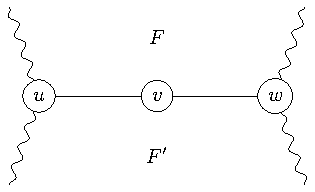
\includegraphics{prelim/img/interiorVertexDegree3.pdf}
%\caption{The notation as described in the proof \label{fig:interiorVertexDegree3}
%}
%\end{figure}

\subsection{Incomplete proofs}
\begin{thrm}[Existence of a eligible path]
\label{th:eligExistence}
When the algorithm's invariant (\ref{i:SWandSE} - \ref{i:last}) are satisfied and the cycle $\C$ is separating then there exist a \emph{eligible} internal path.
\end{thrm}
\begin{proof}
We will first show that there always exists an internal path $\P$. We will then show that a internal path can be found that satisfies conditions $(E1) - (E4)$.

In the proof we will often use that a

Let us first note that if the cycle $C$ is separating (i.e has a non-empty interior), there is at least one interior vertex $v$. Since the triangulation of a $n$-gon is $2$-connected there are two ways to go from $v$ to (say) $S_r$. Hence there is an internal path $\P_0$.
%TODO this is not true, luckily we can use the connections to cyle lemma

If this path does not satisfy \ref{e:noS} we can use the following construction. The other vertex where $P_0$ intersects $\C$ is not $S_r$. Let us call this vertex $x$ and it's neighbor on the path $y$. The vertex $x$ might be $N_b$ or $S_b$ but can't be both, hence it has at least one neighbor $z$ on the cycle that is not $S_r$. Because the triangulation of a $n$-gon is internally maximally planar we have that $yz$ is an edge. Now $xyz$ is an internal path satisfying \ref{e:noS}. See also figure \ref{fig:E1}, here we made a choice on which side of $y$ the vertex $z$ lies, but this choice can be made without losing generality.

Hence we have now constructed, or already had, a path that satisfies \ref{e:noS}. Let us for the remainder of the proof denote this path by $\P_1$.


\begin{figure}[ht]
\centering
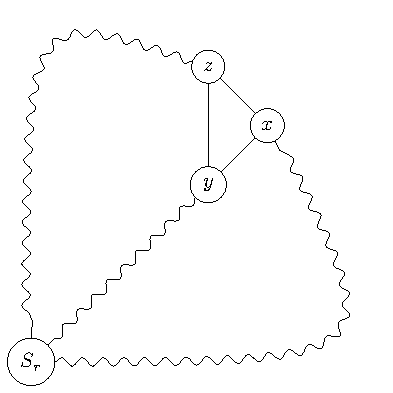
\includegraphics[]{algo/img/E1}
\caption{Constructing a path satisfying \ref{e:noS} \label{fig:E1}}
\end{figure}

\paragraph{There is a path that also satisfies (E2)}
If $\P_1$ satisfies (E2) we set $\P_2 = \P_1$ otherwise we will create a path that satisfies (E1) and (E2).
If the path $\P_1$ does not satisfy $(E2)$ \footnote{which will be the case if the above construction has been used} then there are two possibilities  a) $\P_1$ does not have interior vertices and/or b) $[v,v']$ does not have interior vertices. If a) would be true the existence of $P_0$ would contradict Invariant \ref{i:noChords}. Hence the only problem can be that $b)$ occurs.

If $v=N_b$ and $v'=S_b$ we have found a separating triangle given by $S_rN_bS_b$ \footnote{this is the cycle $\C$ which is separating} in original graph. Hence at least one of $v$ or $v'$ is not $N_b$ or $S_b$. If we call this vertex $x$ its neighbor on the path $y$ and it's neighbor outside $[v,v']$ $z$. We see that by the interior of $\C$ being maximally planar $yz$ must be an edge. If we now adapt $P_1$ by replacing $yx$ by $yz$ we have made $[v,v']$ one vertex longer and hence created a path satisfying \ref{e:longBorders}. In figure \ref{fig:E2} we show this procedure in two cases. Executing this procedure does not change that $S_r$ is not one of the endpoints of the path. Hence we have now created a path $\P_2$ that satisfies \ref{e:noS} and \ref{e:longBorders}.

\begin{figure}
    \centering
    \begin{subfigure}[b]{0.45\textwidth}
        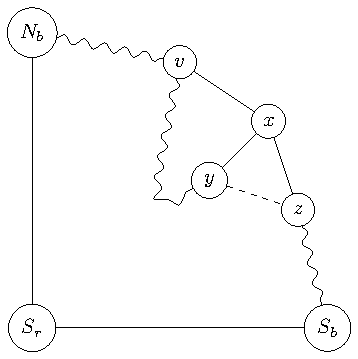
\includegraphics[width=\textwidth]{algo/img/E2general}
        \caption{The general case. Note that $x=v'$.}
    \end{subfigure}
    ~
    \begin{subfigure}[b]{0.45\textwidth}
        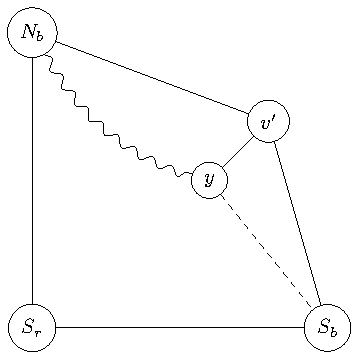
\includegraphics[width=\textwidth]{algo/img/E2spec}
        \caption{A specific case. Note now that $N_b=v, v'=x$ and $S_b=z$}
    \end{subfigure}

    \caption{Creating a path satisfying \ref{e:longBorders}. The dotted line is the edge we take in the new path $\P_2$}\label{fig:E2}
\end{figure}

\newcommand{\intvv}{\ensuremath{[v,v']\setminus{v,v'}}}
\newcommand{\intP}{\ensuremath{\P\setminus{v,v'}}}

\paragraph{There is a path that also satisfies (E3)}
If $\P_2$ satisfies $(E3)$, we take $\P_3 = \P_2$. Otherwise we will remedy the defect. We separate five different cases of offending edges. All of the five cases will be easy to remedy giving a path $\P'_2$ still satisfying \ref{e:noS} and \ref{e:longBorders} such that $\C_{\P'_2}$ is strictly contained in $\C_{\P_2}$ %Q what is the right version of smaller here?
\begin{enumerate}
 \renewcommand*{\labelenumi}{\alph{enumi})}%
 \renewcommand*{\theenumi}{\alph{enumi})}%
 \item edges from \intvv to $\intvv$
 \item edges from $\intP$ to $\intP$
 \item edges incident to $v$ or $v$ and some other vertex on $\C_{\P_2}$
 \item edges from $[v,v']$ to some internal vertex
 \item edges from $\intP$ to some internal vertex
\end{enumerate}

The existence of an edge as in a) is forbidden by Invariant \ref{i:noChords}. If b) occurs we can simply shortcut our original path $\P_2$ with this edge. If c) occurs this edge can't go to another vertex in $[v,v']$ since that would offend Invariant \ref{i:noChords}. Hence they go to a vertex in $\P_2$ and we can shortcut the path as in b).

If d) occurs we simply make a new path and if e) occurs we take a slightly adapted interior path. See figures

%TODO pictures

Since all of the moves shrink $\C_{\P_2}$ while keeping \ref{e:noS} and \ref{e:longBorders} intact and we can't infinitely shrink this means at a certain point no more moves are available. Since every offending edges allows a move this means that there are no more offending edges. Hence this version of $\P'_2$ satisfies \ref{e:crossingEdges}. For the final step of the proof we take $\P_3 = \P'_2$.

%TODO formulate repetition argument nicly

\paragraph{There is a path that also satisfies \ref{e:noNewChord}}
Suppose that $\P_3$ does not satisfy \ref{e:noNewChord}. Then we can just take the would be interior edge and take this for a new path. This is again a finite procedure reducing the sum of $|\P_3| -|[v,v']|$. In the end we have a path satisfying \ref{e:noS} - \ref{e:noNewChord}.

%TODO picturse, why dont we lose E1-E3


\end{proof}
